% !TeX spellcheck = fr_FR
\chapter{Chapitre 5 : Conception}
\label{chap:5}

\section{Architecture LSTMB avec TFR}
\label{sec:5.1}

\begin{figure}[H]
	\centering
	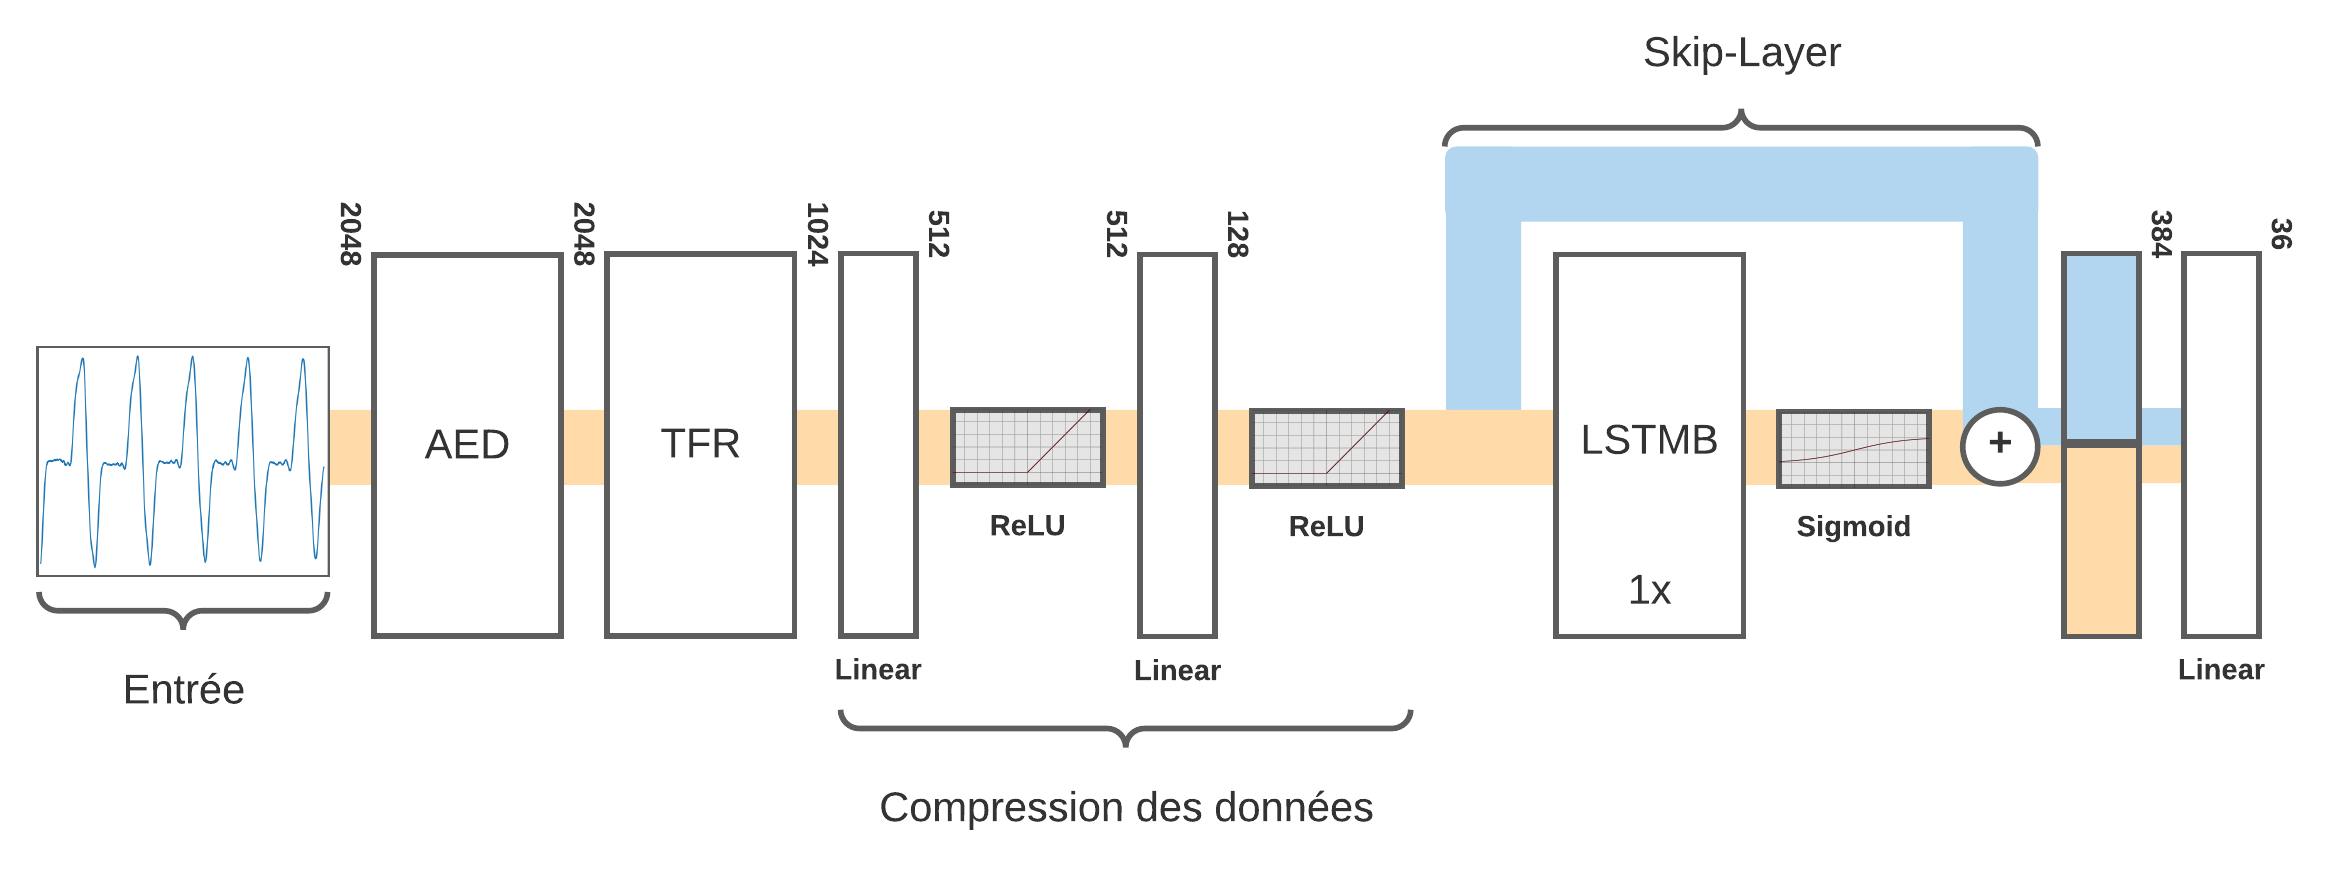
\includegraphics[width=1\linewidth]{lstmb_fft}
	\caption[Architecture LSTMB avec TFR]{Architecture LSTMB avec TFR. Source : Réalisé par \textsc{Küenzi} Jean-Daniel}
	\label{fig:lstmb_fft}
\end{figure}

Dans cette thèse je vais uniquement présenter les architectures avec la \gls{tfr} car ce sont celles qui ont fourni les meilleurs résultats. Les architectures que j'ai utilisées avec les données discrètes se trouvent en annexe. Il s'agit tout simplement de la même architecture sans la \gls{tfr} et avec des couches de normalisation par lots (voir \autoref{sec:5.5}) en plus.

\section{Auto-encodeur débruiteur (AED)}
\label{sec:5.2}

J'ai appris la connaissance de l'\gls{aed} en lisant le document "Autoencoders" \parencite{bank_autoencoders_2021}. Je voulais trouver un moyen de retirer le bruit de mes données de manière rapide (nécessaire pour l'utilisation en temps réel) et sans avoir à passer par des filtres à convolution. Il était important de pouvoir réduire le bruit dans un signal dans le cas où nous n'utilisons pas du matériel spécialisé dans le traitement audio. De plus, je me suis dit que cela pourrait aider à réduire les différents effets, comme le gain ou la distorsion, que nous pouvons ajouter sur le signal. Cette réduction pourra donc aider le modèle à prédire plus facilement l'accord ou la note. En temps réel et dans le monde de l'audio, la latence que l'on est prêt à accepter est en dessous de cinq millisecondes pour le traitement du son (les calculs). D'où la nécessité d'avoir une méthode rapide et simple.

Le but d'un \gls{aed} est de reconstruire les données originales non bruitées à partir de données bruitées. Pour ce faire, on va volontairement bruiter les données qui vont servir d'exemples lors de l'entrainement en rajoutant du bruit blanc gaussien $X\rightarrow\tilde{X}$ et en entrainant l'\gls{aed} à reconstruire les données non bruitées en calculant la perte $L(\tilde{X}, X)$.

Il existe plusieurs types d'auto-encodeurs et différentes architectures, mais j'ai décidé d'opter pour une architecture profonde en bottle-neck afin de ne pas perdre trop de temps en traversant le réseau. Comme nous voulons prédire en temps réel, il doit y avoir le moins de temps possible passé à traverser le réseau.

Lorsque le signal va passer dans l'\gls{aed}, il va être séparé un huit vecteurs de taille 256, puis il sera reconstruit en un vecteur de taille 2048 à la fin, juste avant d'être normalisé à nouveau. On effectue une séparation, car l'architecture dense utilisée est plus efficace pour réduire le bruit sur des petites tailles de vecteurs que sur des grandes.

\subsection{Architecture}

\begin{figure}[H]
	\centering
	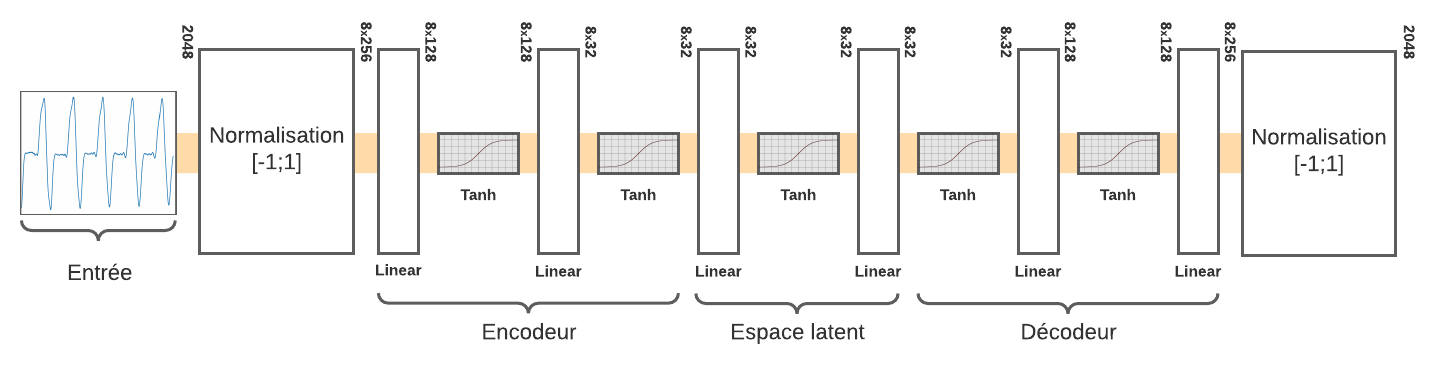
\includegraphics[width=1\linewidth]{aed}
	\caption[Architecture AED]{Architecture AED. Source : Réalisé par \textsc{Küenzi} Jean-Daniel}
	\label{fig:aed}
\end{figure}

\subsection{Bruit blanc gaussien}

Le bruit blanc gaussien est un type de bruit qui est utilisé pour corrompre des données et qui est largement utilisé dans le monde des \gls{aed}. Il est très intéressant, car sa puissance est uniforme sur toute la largeur de bande de fréquences et il suit une loi de distribution normale (gaussienne). Le bruit qui a été ajouté a une moyenne de zéro et un écart type de zéro virgule trois. Dans le monde des signaux, il peut être comparable à un bruit de souffle constant assez fort.

\subsection{Normalisation}

Lorsque le signal va passer à travers l'\gls{aed}, il va être normalisé à son entrée puis à sa sortie. La normalisation des données est d'une importance capitale pour le réseau, cela va lui permettre de ne pas apprendre les amplitudes des signaux et va lui permettre de se concentrer sur d'autres caractéristiques. Aussi, la normalisation va aidée l'\gls{aed} à se faire sa propre représentation des données dans son espace latent et à converger plus rapidement.

La normalisation effectuée est une Min-Max avec une plage entre moins un et un. Son avantage est qu'elle est rapide à faire et elle va conserver le rapport entre les différentes amplitudes du signal (la forme du signal reste inchangée). Avec un signal discret $Y$ et le signal discret normalisé $Y'$, la normalisation appliquée peut être définie comme :

{\Large
	\setlength{\abovedisplayskip}{-0.5cm}
	\begin{align*}
		Y' = 2\frac{Y-\text{min}(Y)}{\text{max}(Y)-\text{min}(Y)}-1
	\end{align*}
}

\subsection{Espace latent}

L'espace latent est une représentation compressée des données que le réseau va apprendre de lui-même. Lors de l'entrainement, il va apprendre à extraire les caractéristiques qui lui semble les plus pertinentes et va ensuite les utiliser afin de reconstruire les données non bruitées.

\subsection{Perte de reconstruction}

Pour un auto-encodeur, on parle de perte de reconstruction pour signifier la différence entre les données attendues et les données reconstruites. La fonction que j'ai utilisée pour calculer ma perte de reconstruction est l'erreur quadratique moyenne. Avec $Y_{i}$ la sortie actuelle, $\hat{Y}_{i}$ la sortie attendue et $N$ la taille. L'erreur quadratique moyenne peut être définie comme :

{\Large
	\setlength{\abovedisplayskip}{-0.5cm}
	\begin{align*}
		E[\overrightarrow{W}] = \frac{1}{N}\sum_{i=0}^{N-1}{(Y_{i} - \hat{Y}_{i})^2}
	\end{align*}
}

\section{Transformée de Fourier rapide (TFR)}
\label{sec:5.3}

Une fois que le signal est passé par l'\gls{aed}, on va effectuer une \gls{tfr} afin de récupérer son spectre. Mais avant de faire la \gls{tfr}, nous allons multiplier le signal par une fenêtre de Hamming afin de réduire la fuite spectrale et de faciliter ainsi l'apprentissage au réseau.

\subsection{Composante du spectre continu}

Comme vu dans la \autoref{sec:2.8}, nous nous intéressons uniquement à la partie du spectre continu. Donc lorsque que nous effectuons une \gls{tfr} avec une fenêtre de taille $N$ nous allons uniquement prendre en compte les $N/2$ premiers coefficients de Fourier. Cette réduction de moitié permet au réseau d'être plus précis sur ses prédictions et plus rapide. Comme la \gls{tfr} retourne des nombres complexes, c'est le module de ses nombres que l'on va passer au réseau (voir \autoref{sec:2.8}).

\subsection{Normalisation}

Une fois la \gls{tfr} faite, nous allons normaliser les données afin que la valeur des amplitudes ne soit pas un facteur que le réseau doivent apprendre. Finalement, tout ce qui nous intéresse c'est uniquement de connaitre les fréquences et non leurs amplitudes. On va donc pouvoir normaliser le spectre obtenu afin de faciliter au réseau l'apprentissage et la prédiction.

La normalisation effectuée est une Min-Max avec une plage entre zéros et un. Son avantage est qu'elle est rapide à faire et elle va conserver le rapport entre les différentes amplitudes du spectre. Avec un signal discret $Y$ et le signal discret normalisé $Y'$, la normalisation appliquée peut être définie comme :

{\Large
	\setlength{\abovedisplayskip}{-0.5cm}
	\begin{align*}
		Y' = \frac{Y-\text{min}(Y)}{\text{max}(Y)-\text{min}(Y)}
	\end{align*}
}

\section{Compression des données}
\label{sec:5.4}

Comme pour l'\gls{aed}, cette couche va permettre au réseau de se faire sa propre représentation des données qu'il reçoit de la \gls{tfr}. Lors de l'entrainement, il va apprendre à extraire les caractéristiques qui lui semblent importantes. Cette couche est ajoutée afin de permettre aux données de traverser plus rapidement le réseau sans perdre pour autant la précision.

\section{Normalisation par lots}
\label{sec:5.5}

La normalisation par lots ou (\textit{Batch Normalization} en anglais) est une technique décrite dans le document "Batch Normalization: Accelerating Deep Network [...]" \parencite{ioffe_batch_2015}. Le principe est de rajouter des couches qui vont aider à mieux coordonner la mise à jour des poids lors de la rétropropagation du gradient. Elle rend notamment le réseau moins dépendant du paramétrage initial comme le taux d'apprentissage et la génération aléatoire des poids. Elle permet aussi dans certains cas de ne pas avoir besoin de recourir à des couches de dropout.

En apprentissage profond, lors de la rétropropagation du gradient, on corrige les poids d'une couche à partir d'une estimation de l'erreur en supposant que les poids des couches précédentes sont fixes. Mais finalement comme nous mettons à jour toutes les couches du réseau simultanément cette supposition est fausse. Cela nous oblige à faire attention aux paramètres d'initialisations du réseau et ralentit l'entrainement en nous contraignant à utiliser un petit taux d'apprentissage. Dans le document \parencite{ioffe_batch_2015}, ce problème est nommé "Changement de Covariable Interne" (\textit{Internal Covariate Shift} en anglais).

La normalisation par lots va nous aider à régler ce problème en normalisant les entrées des couches par mini-lots (\textit{mini-batchs} en anglais) pour avoir une moyenne de zéro et un écart type de un. Cette normalisation permet au réseau durant la rétropropagation du gradient de mieux régulariser l'erreur et de rendre la mise à jour des poids moins propice à varier de manière drastique.

Cette problématique de réduction du changement de covariable interne reste encore discutée. D'autres études comme "How Does Batch Normalization Help Optimization?" \parencite{santurkar_how_2019} estiment que la normalisation par lots aide l'entrainement du réseau en rendant la descente de gradient plus lisse et simplifie donc la convergence du réseau.

Il est aussi possible de permettre à la couche de normalisation d'apprendre deux paramètres, $\beta$ et $\gamma$. Généralement cela se fait beaucoup, car normaliser les entrées des couches peut modifier la représentation de la couche. Ces deux paramètres permettent de s'assurer de pouvoir retrouver la transformation identité (la réelle représentation).

Avec $x$ les entrées, $E[x]$ l'erreur pour chaque entrée, $\text{Var}[x]$ l'écart type pour chaque entrée, $\epsilon$ une valeur ajoutée pour la stabilité numérique, $\beta$ et $\gamma$ les deux paramètres apprenables. PyTorch \parencite{noauthor_batchnorm1d_nodate} définit la normalisation par lots comme :

{\Large
	\setlength{\abovedisplayskip}{-0.5cm}
	\begin{align*}
		y = \frac{x - E[x]}{\sqrt{\text{Var}[x] + \epsilon}}\times\gamma+\beta
	\end{align*}
}

J'ai utilisé les couches de normalisation par lots lors de la prédiction avec les données discrètes (sans \gls{tfr}) car cela avait un impacte non négligeable sur la précision des modèles. Mais lors de l'utilisation avec les données de la \gls{tfr} j'ai constaté une perte de précision. Les couches de normalisation par lots sont ajoutées après les couches denses et les couches de convolution mais avant la fonction d'activation ReLU qui est non linéaire, comme précisé dans le document \parencite{ioffe_batch_2015}. Les tableaux ci-dessous représentent les différences d'entrainements de l'architecture LSTMB sans \gls{tfr} (voir \autoref{app:1}) avec et sans couches de normalisation par lots.

\begin{table}[H]
	\centering{
		\begin{tabular}{l c c}
			\hline
			\multicolumn{3}{c}{\textbf{Sans la normalisation par lots}} \\
			\multicolumn{3}{c}{epochs = 50, $\eta$ = 0.005, nombre d'entrainements = 10} \\
			\hline
			\textbf{Données} & \textbf{Précision moyenne \%} & \textbf{Ecart type \%}\\
			\hline
			Entrainement & 98.19 & 0.43 \\
			Validation & 88.36 & 0.51 \\
			\hline
		\end{tabular}
		\caption[Entrainement sur données discrètes sans la normalisation par lots]{Entrainement sur données discrètes sans la normalisation par lots. Source : Réalisé par \textsc{Küenzi} Jean-Daniel}
		\label{tab:without_batchnorm}
	}
\end{table}

\begin{table}[H]
	\centering{
		\begin{tabular}{l c c}
			\hline
			\multicolumn{3}{c}{\textbf{Avec la normalisation par lots}} \\
			\multicolumn{3}{c}{epochs = 50, $\eta$ = 0.005, nombre d'entrainements = 10} \\
			\hline
			\textbf{Données} & \textbf{Précision moyenne \%} & \textbf{Ecart type \%}\\
			\hline
			Entrainement & 99.91 & 0.02 \\
			Validation & 92.45 & 0.54 \\
			\hline
		\end{tabular}
		\caption[Entrainement sur données discrètes avec la normalisation par lots]{Entrainement sur données discrètes avec la normalisation par lots. Source : Réalisé par \textsc{Küenzi} Jean-Daniel}
		\label{tab:with_batchnorm}
	}
\end{table}

En observant les résultats, on constate bien l'efficacité de ces couches de normalisation par lots. Avec les mêmes paramètres d'initialisation, le modèle a convergé beaucoup plus rapidement et l’on a ainsi gagné un peu plus de quatre pour cent de précision moyenne sur l'ensemble de validation.

\section{Cellule LSTM Bidirectionnelle (LSTMB)}
\label{sec:5.6}

Une cellule \gls{lstmb} est en fait composé de deux cellules \gls{lstm}. Une qui va propager $h_t$ vers l'avant et une qui va le propager vers l'arrière. On peut voir sa comme recevoir les informations du passé et du futur à la fois. Une cellule LSTM classique utilise $h_{t-1}$ (passé) pour produire $h_t$. Une cellule \gls{lstmb} va à la fois utiliser $h_{t-1}$ et $h_{t+1}$ (futur) pour produire $y_t$ qui est notre sortie. En fait $y_t$ est tout simplement une concaténation (parfois accompagné d'une fonction d'activation) des sorties $h_t$ des deux cellules (voir \autoref{fig:bidirectional_lstm}). Comme on récupère la sortie des deux cellules et qu'on concatène, on à plus de données à la sortie qu'à l'entrée.

Donc dans notre cas, on peut voir qu'on a un vecteur de taille 128 à l'entrée de la cellule et on aura donc un vecteur de taille 256 à sa sortie, on a augmenté la taille de nos données par un facteur deux.

\subsection{Architecture}

\begin{figure}[H]
	\centering
	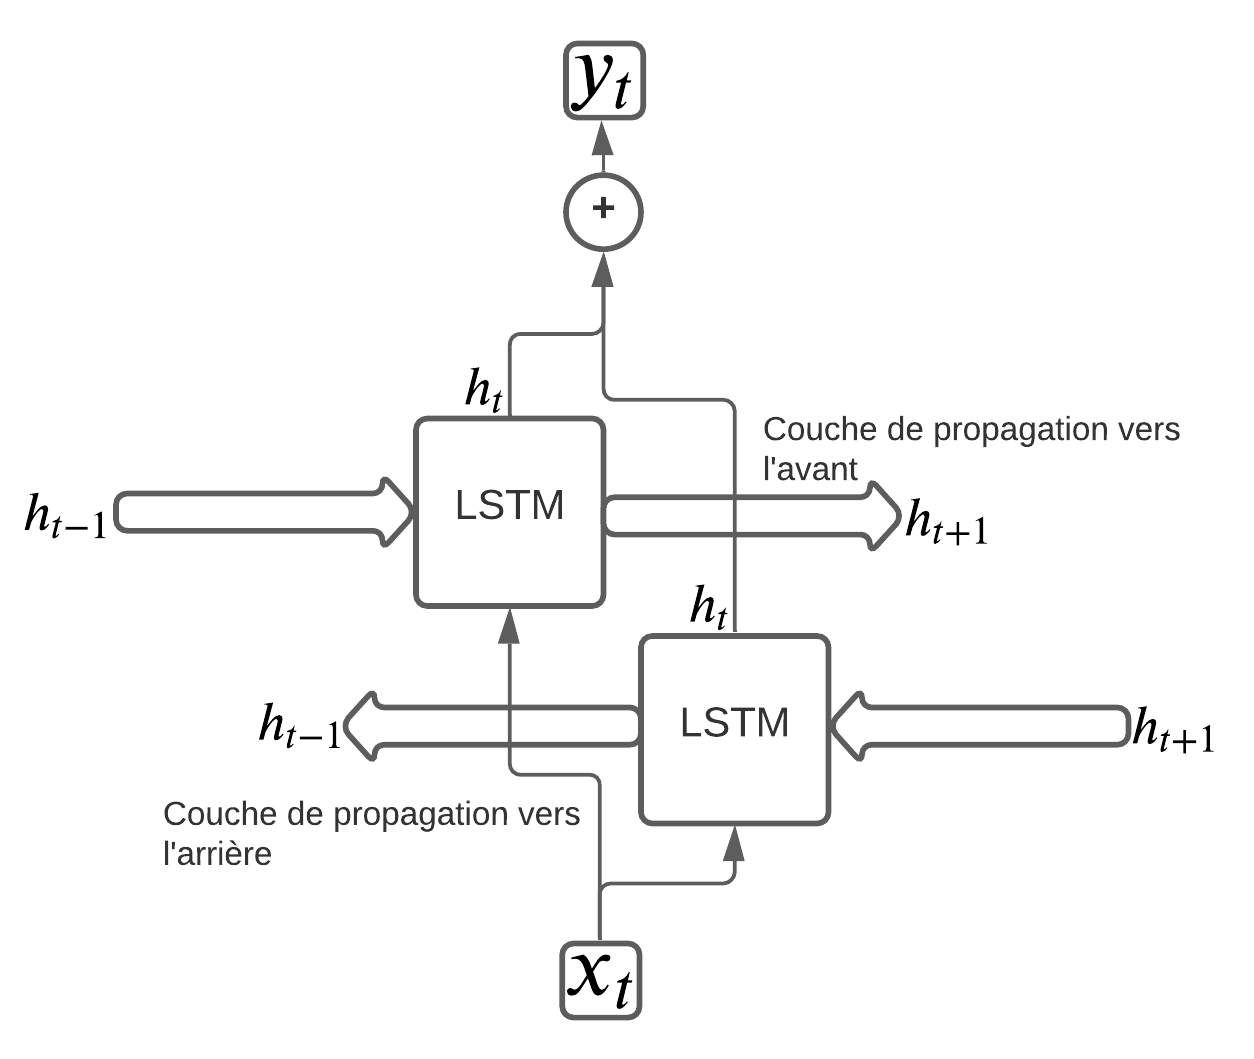
\includegraphics[width=0.7\linewidth]{bidirectional_lstm}
	\caption[Cellule LSTM Bidirectionnelle]{Cellule LSTM Bidirectionnelle. Source : Réalisé par \textsc{Küenzi} Jean-Daniel}
	\label{fig:bidirectional_lstm}
\end{figure}

\section{Skip-Layer}
\label{sec:5.7}

La Skip-Layer est en fait une technique utilisée où, comme son nom l'indique, on va éviter des couches. Comme on peut le voir sur la \autoref{fig:lstmb_fft}, une copie des données vont êtes prises avant de traverser la cellule \gls{lstmb} et vont ensuite être concaténée à sa sortie. La skip-layer va permettre aux couches suivantes d'apprendre également des données qui se trouvent avant la cellule \gls{lstmb}. Elle aide aussi pour la rétropropagation du gradient, notamment en aidant à éviter le problème du gradient de fuite. La Skip-Layer est beaucoup utilisée dans les architectures modernes.

\section{Fonction de coût}
\label{sec:5.8}

La fonction de coût que j'ai utilisé est l'entropie croisée (\textit{cross-entropy} en anglais). PyTorch \parencite{noauthor_crossentropyloss_nodate} utilise une combinaison de la fonction de perte logarithmique de vraisemblance négative (\textit{Negative Log-Likelihood Loss} en anglais) et de la fonction Logarithmique Softmax (\textit{Log-Softmax} en anglais), qui est tous simplement le logarithme de la fonction softmax. En pratique, on préfère l'utilisation de la fonction log-softmax plutôt que la fonction softmax. Elle est plus utilisée, car la fonction log-softmax aide le réseau en assurant une stabilité numérique de l'erreur. Elle ne va jamais devenir infiniment petite. Aussi, de par sa nature exponentielle elle inflige des pénalités beaucoup plus lourdes que la softmax (qui est linéaire) pour les classes incorrectes, et aide donc le réseau à converger plus vite. Pour finir, elle est optimisée pour effectuer moins de calculs que la softmax durant la descente de gradient. Avec $x$ un tenseur de valeurs réelles. PyTorch définit la log-sofmax comme :

{\Large%
	\setlength{\abovedisplayskip}{-0.5cm}
	\begin{gather*}
		\text{LogSoftmax}(x_i) = \text{log}(\frac{\text{exp}(x_i)}{\sum_{j}{\text{exp}(x_j)}})
	\end{gather*}
}%

et donc avec $x$ un tenseur de valeurs réelles qui représente la sortie du réseau et $y$ un tenseur correspondant aux classes correctes attendues, PyTorch \parencite{noauthor_crossentropyloss_nodate} définit l'entropie croisée comme

{\Large%
	\setlength{\abovedisplayskip}{-0.5cm}
	\begin{gather*}
		\text{L}(x, y) = -x_y + \text{log}(\sum_{j}{\text{exp}(x_j)})
	\end{gather*}
}%

